\graphicspath{{fake_results/}}
\subsection{System Usability Scale Results}

The system usability scale (SUS) contains ten statements all related to the user experience that are scored from strongly disagree to strongly agree. These answers correspond to the numbers 0 to 4, and a final score is calculated using \autoref{eq:SUS_score}.

\begin{equation}
	\frac{(\sum\limits_{n=1}^{10} \sum\limits_{p=1}^{P} S) \cdot 2.5 }{P}
	\label{eq:SUS_score}
\end{equation}

where $ n $ is statement, $ p $ is participant number, $ P $ is number of participants, and $ S $ is score. It is multiplied by $2.5$ to get a score between $ 0 $ and $ 100 $ to compare with as a percentile. %NOTE: we should probably change this to median and quartiles, but I don't know if there is some official thing

The first statement does not necessarily apply to most of the test participants as they can not expect to use the system again, however the authors decided the question was still relevant to gauge whether the participants enjoyed the experience. 

\begin{figure}[h]
\centering
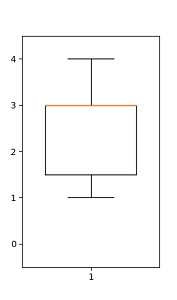
\includegraphics[width=0.32\textwidth]{1.png}
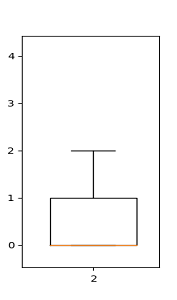
\includegraphics[width=0.32\textwidth]{2.png}
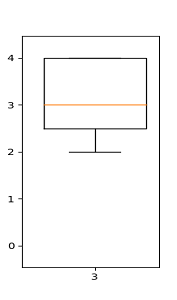
\includegraphics[width=0.32\textwidth]{3.png}
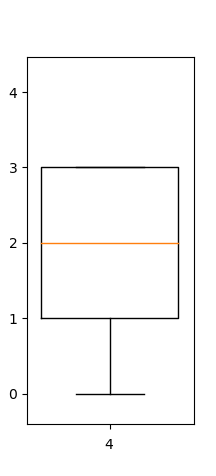
\includegraphics[width=0.32\textwidth]{4.png}
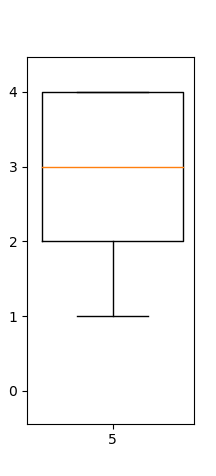
\includegraphics[width=0.32\textwidth]{5.png}
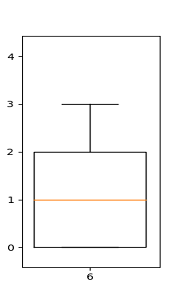
\includegraphics[width=0.32\textwidth]{6.png}
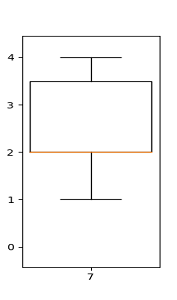
\includegraphics[width=0.32\textwidth]{7.png}
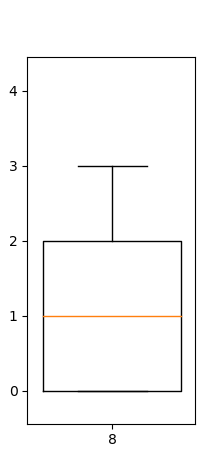
\includegraphics[width=0.32\textwidth]{8.png}
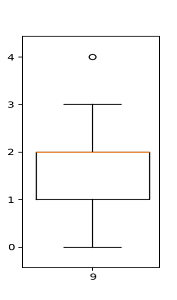
\includegraphics[width=0.32\textwidth]{9.png}
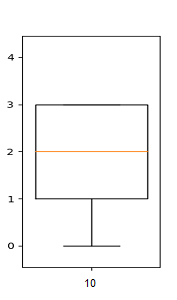
\includegraphics[width=0.32\textwidth]{10.png}
\caption{Answers to statements from the SUS}
\label{fig:one}
\end{figure}

%I am familiar with VR or VR controls
The median score was 67.5, with the first quartile scoring 45 and the third scoring 86.25. %Note: 68 is the american average SUS score - is this result or discussion? Probably discussion

There were also X other questions following the standard SUS that were meant to gauge user familiarity and experience. These were concerned with age, gender, and familiarity with VR controls. 

\begin{figure}[H]
	\centering
	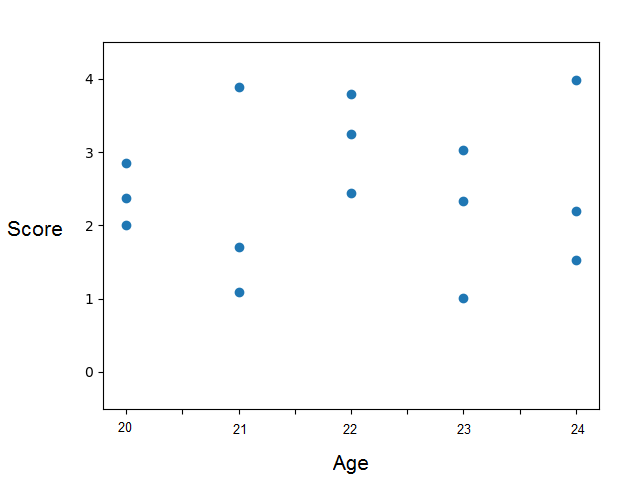
\includegraphics[width = 0.48\textwidth]{age.png}
	\caption{Mean scores plotted as a function of participant age}
	\label{fig:age}
\end{figure}

\autoref{fig:age} shows the participants' scores plotted as a function of their age. Linear regression returns $y = 0.03x + 2.06$. $R^2$ returns value close to 1 ($0.99$). Mean scores from both genders were also close ($ 3.01 $ and $ 2.99 $). 

\begin{figure}[H]
	\centering
	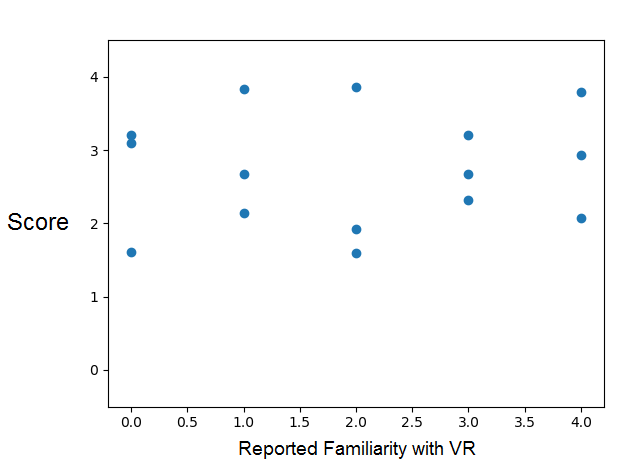
\includegraphics[width = 0.48\textwidth]{Familiarity.png}
	\caption{Mean scores plotted as a function of participants' familiarity with VR tools}
	\label{fig:fam}
\end{figure}

Finally, \autoref{fig:fam} shows participants' mean scores plotted as a function of their self reported familiarity with VR. This question was to gauge whether participants had trouble with VR itself or the system, thus if there was an obvious learning curve for those inexperienced with VR and whether that affected their experience. Linear regression yielded $y = -0.05x + 3$, and $R^2$ returns close to 1 yet again ($R^2=0.89$).